\chapter{Projections for the Proposed Measurements}
\label{chap:reach}
In this work we propose to measure the neutron's DVCS beam-spin asymmetry in 
the following two channels:
\begin{enumerate}
   \item Tagged n-DVCS: $D\,+\,\gamma^{*}  \longrightarrow 
      \gamma\,+\,(n)\,+\,p$
   \item Fully exclusive n-DVCS: $D\,+\,\gamma^{*}  \longrightarrow \gamma\,+\, 
      n \,+\,p$
\end{enumerate}

To demonstrate the experimental feasibility and to extract projections for our 
proposed measurements, we present here a simulation study using a realistic 
n-DVCS event generator and the official simulation-reconstruction chain of 
CLAS12 spectrometer upgraded with BONuS12 RTPC. 


\section{Monte-Carlo Simulation}
An event generator for DVCS/BH and exclusive $\pi^0$ electroproduction on the 
neutron inside a deuterium target has been developed \cite{ahmed}. The DVCS 
amplitude is calculated according to the BKM formalism \cite{Belitsky:2001ns}, 
while the GPDs have been taken from the VGG model 
\cite{PhysRevD.60.094017,Guidal:2004nd}. The Fermi-motion distribution is 
calculated with the Paris potential \cite{PhysRevC.21.861}.

The output of the event generator was fed through CLAS12 official simulation 
(GEMC 4.3.0)~\cite{clas12-gemc} and reconstruction (COATJAVA 
5b.7.4)~\cite{clas12-coatjava} chain, to simulate the detectors' acceptance and 
resolutions for the following final state particles, electrons, photons, 
and neutrons, within the proposed experimental setup of Run Group F. Spectator 
protons are reconstructed with a fastMC that was developed based on the 
performance of the eg6 CLAS run.

\section{Particle Identification}

The final state of neutron Tagged-DVCS event consists of three particles: an 
electron, a proton, and a real photon, while in addition to these particles a 
neutron is required to be detected in the fully exclusive neutron's DVCS 
events. To identify the DVCS events, we first identify the different particles 
of interest. Then, events with three and four detected final-state particles 
will be further filtered by imposing the energy-momentum conservation laws.

For the identification of the different final state particle we use the 
official CLAS12 Event-Builder~\cite{eventbuilder}. In the following subsections 
we detail the main requirement for the different particles. 

\subsection{Electron Identification} 
For charged particles in the forward detectors, the Event Builder first assigns 
e$^-$ (PID= 11) or e$^+$ (PID= -11) (depending on the bending direction of the 
reconstructed track in the DC) if a particle satisfies all corresponding HTCC 
and ECAL requirements, and has an associated FTOF hit:
\begin{itemize}
 \item 2.0 photoelectrons in HTCC.
 \item 60 MeV in PCAL.
 \item  5-sigma cuts on a parameterized momentum-dependent sampling fraction 
    where "sampling fraction" is ECAL visible energy deposition 
      (PCAL+Inner+Outer) divided by DC momentum.  
      
\end{itemize}

In addition to these initial selections cuts, some regions of CLAS12 have to be 
excluded from the analysis to ensure an accurate detection of the different 
particles. For instance, an electron that hits the edge of the EC will have 
only part of its electromagnetic shower contained within the detector. Also, 
the structure of the torus magnet divides CLAS12 into six separate sectors, 
which makes edge effects non-negligible. Figure~\ref{fig:el_kin} shows the 
kinematic distributions of the DVCS electrons being detected and reconstructed 
in the forward detector of CLAS12 spectrometer in terms of the energy as a 
function of the polar angle ($\theta$) and the azimuthal angle ($\phi$) as a 
function of $\theta$. 

\begin{figure}[tp]
\centering
   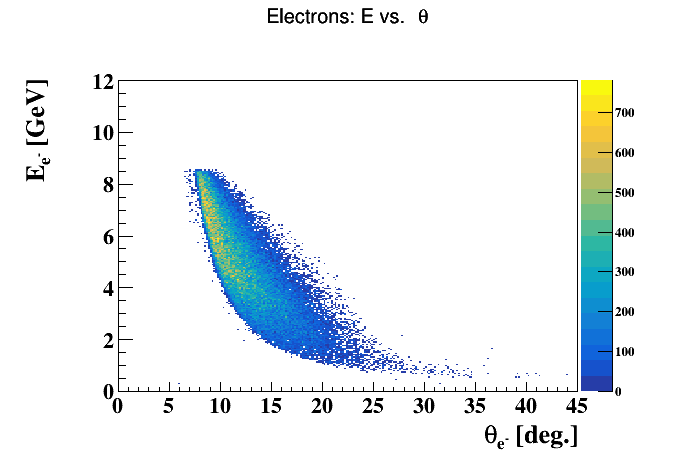
\includegraphics[width=0.48\textwidth,clip,trim=0mm 0mm 0mm 
   20mm]{figs/e_E_theta.png}
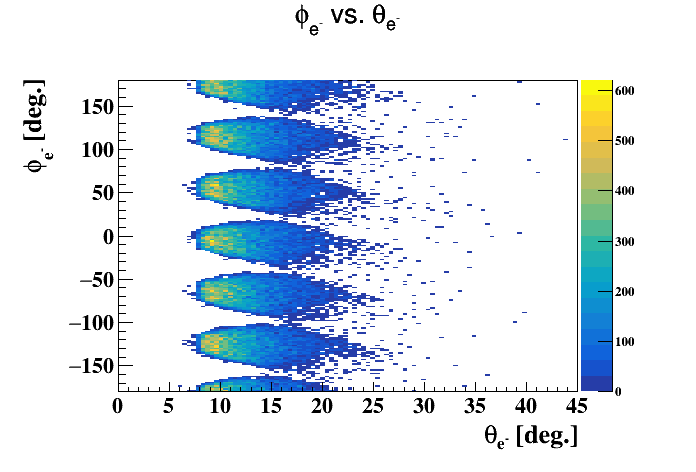
\includegraphics[width=0.48\textwidth,clip,trim=0mm 0mm 0mm 
   20mm]{figs/e_phi_theta.png}
   \caption{Electron's energy as a function of it's polar angle (left) and the 
   azimuthal angle as a function of the polar angle (right), for n-DVCS events.  
   Forward-CLAS12 acceptance and physics cuts are included.}
   \label{fig:el_kin}
\end{figure}
 

\subsection{Proton Identification}
The slow recoiling final state protons will be detected within the BONuS12 
RTPC. As the RTPC is physically within the CLAS12 simulation, but the track 
reconstruction is not finalized yet within CLAS12 reconstruction, we refer to a 
realistic fastmc the reproduces the expected performance of this detector. This 
fastmc has be developed initially from the BONuS6 experiment and tuned very 
precisely after EG6 experiment \cite{eg6_note}, which have used very similar 
RTPCs.  This fastmc smears the proton's kinematics and applies acceptance 
functions. Regarding the smearing, the momentum, polar angle, azimuthal angle, 
and z-vertex of the protons are smeared with Gaussians using the observed 
tracking resolutions of the RTPC (see chapter 2, section 3 in \cite{eg6_note}).  
For the acceptance, the fastmc:
\begin{itemize}
   \item ensures that the proton's track intersects with the cathode.
   \item removes the tracks which pass in the dead area between the two modules 
      of the RTPC.
\item rejects the track if it goes to the upstream end of the target's holder.
\item applies the RTPC's thresholds on the momentum and the polar angle.
\end{itemize} 
We do not specifically apply energy loss and multiple scattering in our fastmc, 
but we do apply resolution effects based on experimental data that include both 
effects. Figure~\ref{fig:proton_kin} presents the kinematic distributions of 
the recoiling final state protons within the active volume of the BONUS12 RTPC. 

\begin{figure}[htb]
\centering
   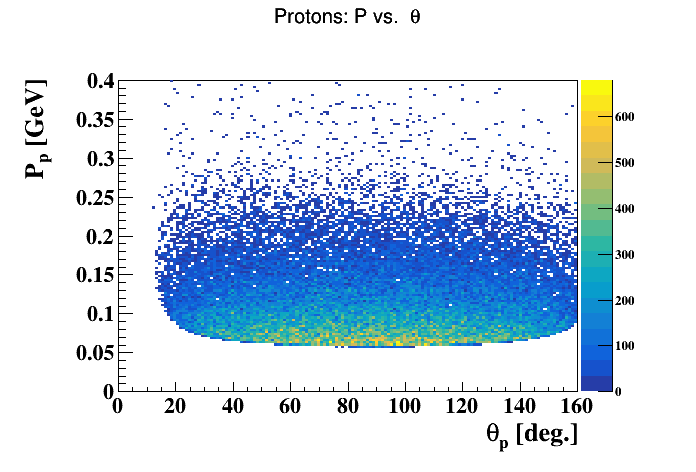
\includegraphics[width=0.48\textwidth,clip,trim=0mm 0mm 0mm 
   20mm]{figs/p_p_theta.png}
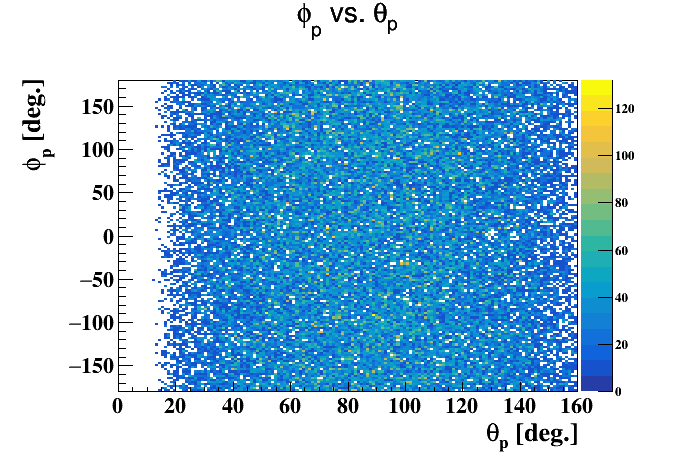
\includegraphics[width=0.48\textwidth,clip,trim=0mm 0mm 0mm 
   20mm]{figs/p_phi_theta.png}
   \caption{Recoiling proton's momentum as a function of it's polar angle 
   (left) and the azimuthal angle as a function of the polar angle (right), 
   from n-DVCS events. BONuS12 RTPC acceptance and physics cuts are included.}
   \label{fig:proton_kin}
\end{figure}
 

\subsection{Neutrals Identification} 

For neutrals, only photon (PID= 22) and neutron (PID= 2112) are considered, and 
particle identification is assigned based on simple beta cut at 0.9. Currently 
only one timing response is used for this, and for ECAL the prioritization is: 
PCAL, EC Inner, EC Outer. The momentum direction is assigned based on the 
neutral's ECAL cluster position and the vertex of the charged particle used to 
determine the start time. For photons, the energy (magnitude of the momentum) 
is calculated from ECAL visible energy and momentum-dependent sampling 
fraction, while for neutrons energy is calculated from beta. For the central 
detector, CND is treated similarly as ECAL, except only neutron PID is assigned 
based on beta and the cut is at 0.8. Figure~\ref{fig:photon_kin} presents the 
kinematic distributions of the neutron-DVCS photons being detected in the 
CLAS12 forward detector. Figure~\ref{fig:neutron_kin} shows similar 
distributions of the detected final state neutrons being detected in both the 
forward and the central detectors of CLAS12 spectrometer. As can be seen from 
figures~\ref{fig:el_kin}, \ref{fig:proton_kin}, ~\ref{fig:photon_kin}, 
~\ref{fig:neutron_kin}, the DVCS electrons and photons are produced very 
forward, which is in a total agreement with our DVCS measurements during the 
6~GeV era of CLAS, while slow recoiling protons are emitted more evenly in the 
polar angle range within the acceptance of the BONuS12 RTPC. The final neutrons 
are mostly emitted above $\theta$ = 40$^{\deg}$, which is outside the 
acceptance of the forward detector of CLAS12 and was the main reason to upgrade 
CLAS12 with the Central neutron Detector during Run Group B to measure the 
neutron DVCS semi-exclusively (E12-11-003).  


\begin{figure}[htb]
\centering
   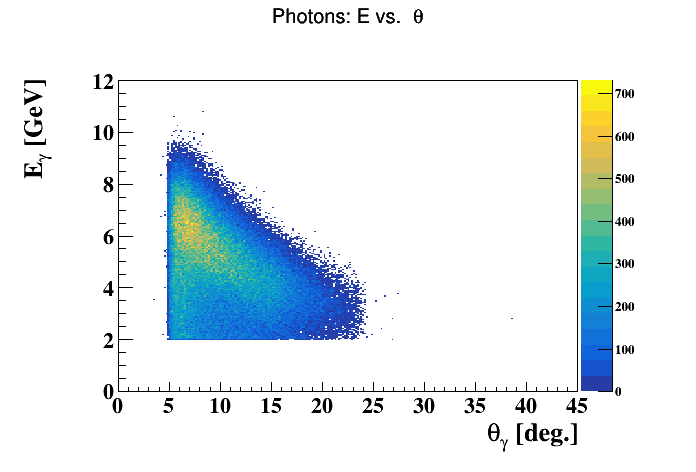
\includegraphics[width=0.48\textwidth,clip,trim=0mm 0mm 0mm 
   20mm]{figs/gamma_E_theta.png}
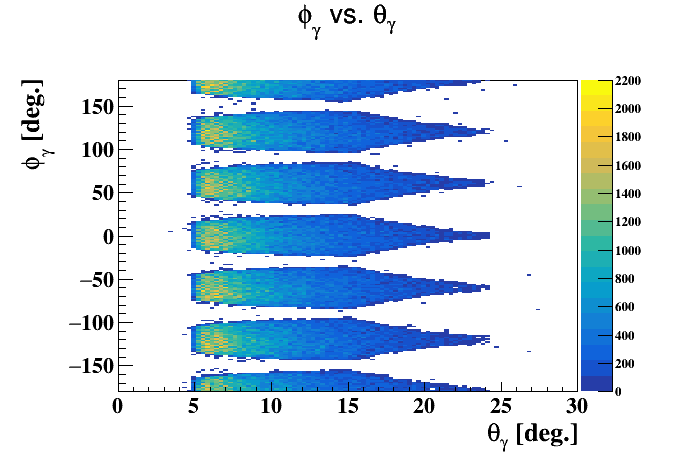
\includegraphics[width=0.48\textwidth,clip,trim=0mm 0mm 0mm 
   20mm]{figs/gamma_phi_theta.png}
   \caption{Photon's energy as a function of it's polar angle (left) and the 
   azimuthal angle as a function of the polar angle (right), for n-DVCS events.  
   Forward-CLAS12 acceptance and physics cuts are included.}
   \label{fig:photon_kin}
\end{figure}
 

\begin{figure}[htb]
\centering
  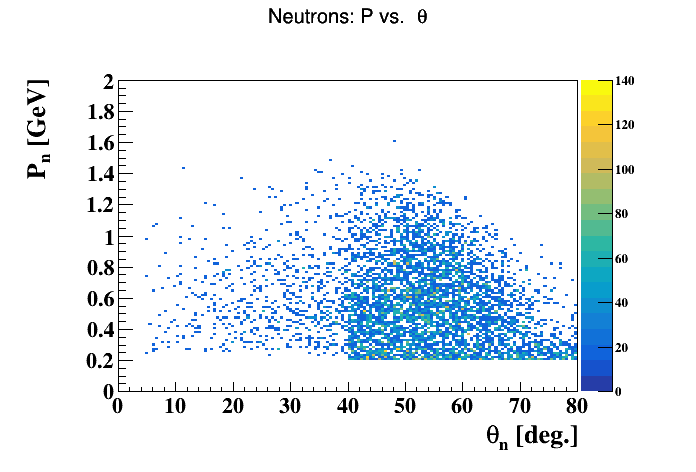
\includegraphics[width=0.48\textwidth,clip,trim=0mm 0mm 0mm 
   20mm]{figs/n_p_theta.png}
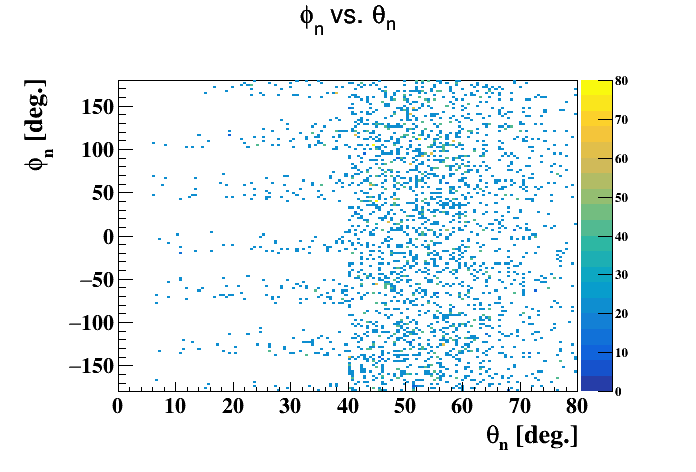
\includegraphics[width=0.48\textwidth,clip,trim=0mm 0mm 0mm 
   20mm]{figs/n_phi_theta.png}
  \caption{Recoiling neutron's momentum as a function of it's polar angle 
  (left) and the azimuthal angle as a function of the polar angle (right), from 
   n-DVCS events. BONuS12 forward and central acceptance and physics cuts are 
   included.}
  \label{fig:neutron_kin}
\end{figure}


\section{Beam-Spin Asymmetry}

The beam spin asymmetry of a longitudinally polarized electron beam on an 
unpolarized target ($A_{LU}$) in each bin of the 108 total bins is defined as:
%
\begin{equation}
  A_{LU} = \frac{1}{P_{B}} \frac{N^{+} - N^{-}}{N^{+} + N^{-} }.
\end{equation}
%
where $P_{B}$ is the beam polarization, and $N^{+}$ and $N^{-}$ are the number 
of events detected with positive and negative electron helicity, respectively.  
The statistical uncertainty of $A_{LU}$ is
%
\begin{equation}
  \sigma_{A_{LU}} = \frac{1}{P_{B}} \sqrt{ \frac{1 - (P_{B}A_{LU})^{2}}{N}}
\end{equation}
%
where $N (= N^{+} + N^{-}) $ is the total number of measured DVCS events in 
each bin.

It is particularly convenient to use the BSA $A_{LU}$ as a DVCS observable, 
because most of the experimental systematic uncertainties, such as 
normalization and efficiencies that appear in the cross sections cancel out in 
the asymmetry ratio. However, some systematic uncertainties remain and they 
still contribute to the measured $A_{LU}$. The main known sources of systematic 
uncertainties are: the DVCS selection cuts, the fitting sensitivity to our 
binning, the beam polarization and the background (non exclusive $\pi^0$) 
acceptance ratio. In the following, we present estimates of the contribution 
from each source based on our prior knowledge during CLAS-eg6 DVCS analysis 
\cite{eg6_note}.

In order to evaluate the systematic uncertainties stemming from the DVCS 
selection cuts, the eg6-analysis was repeated with changing the width of the 
exclusive cuts. The resulting systematic uncertainty to the $A_{LU}$ asymmetry
was around 6$\%$ for the incoherent DVCS channel. Because of the important 
improvement we expect with BONuS12 RTPC in terms of resolutions, we expect this 
uncertainty to be reduced to 4$\%$.

Regarding the sensitivity of the fit results to our binning, the eg6 data were 
binned into two different bins in $\phi$ and the reconstructed asymmetries were 
compared. The associated systematic uncertainty for $A_{LU}$ at $\phi = 90 
^{\circ}$ was found to be of 7.1$\%$. For the proposed measurements, we expect 
to achieve higher statistics and therefore we reduced the expected systematics 
to 3$\%$.
   
The beam polarization will be measured during the experiment by the Hall B 
M\o{}ller polarimeter. This polarimeter measures the angular distribution of 
the M\o{}ller electrons to obtain the beam polarization. The precision of the 
Hall B M\o{}ller polarimeter was measured to be around 3.5$\%$ 
\cite{PhysRevSTAB.7.042802}.  
We assume a 3.5$\%$ systematic uncertainty on the measured 
asymmetries similar to what was achieved during 6 GeV run.

A total systematic contributions is estimated to be around 11\%. To be 
conservative, in particular because expected asymmetries on neutrons are
much smaller than on protons, we used an increased total of 20\% 
systematic uncertainty for our projections. This is added quadratically to the statistical error 
bars in each bin of the reconstructed asymmetry.

\section{Projections}
Once the final state particles being reconstructed and identified after passing 
all the physics and the geometry cuts. We reconstruct two types of neutron DVCS 
events as listed at the beginning of this chapter. Based on the approved  Run 
Group F electron-nucleon running luminosity, a total of 9 million tagged and 
850K fully exclusive neutron DVCS events will be collected during the 35 PAC 
days. In the following two subsections, we present our proposed binning for 
each set of data selection and the projections of the proposed measured 
beam-spin asymmetries.  



\subsection{Tagged n-DVCS Projections}
After identifying the Tagged-neutron DVCS events, i.e., having only one 
electron, one photon, and one proton in the final state, we further filter them 
by imposing the energy-momentum conservation laws.  
Figure~\ref{fig:tagged_exclusive} shows the missing mass squared distribution 
of the identified tagged neutron DVCS events in addition to the missing energy 
distribution of these events. We apply an additional cut on the reconstructed 
missing mass squared to further clean the selected events as shown by the 
vertical red-dashed lines. 

\begin{figure}[htb]
  \centering
    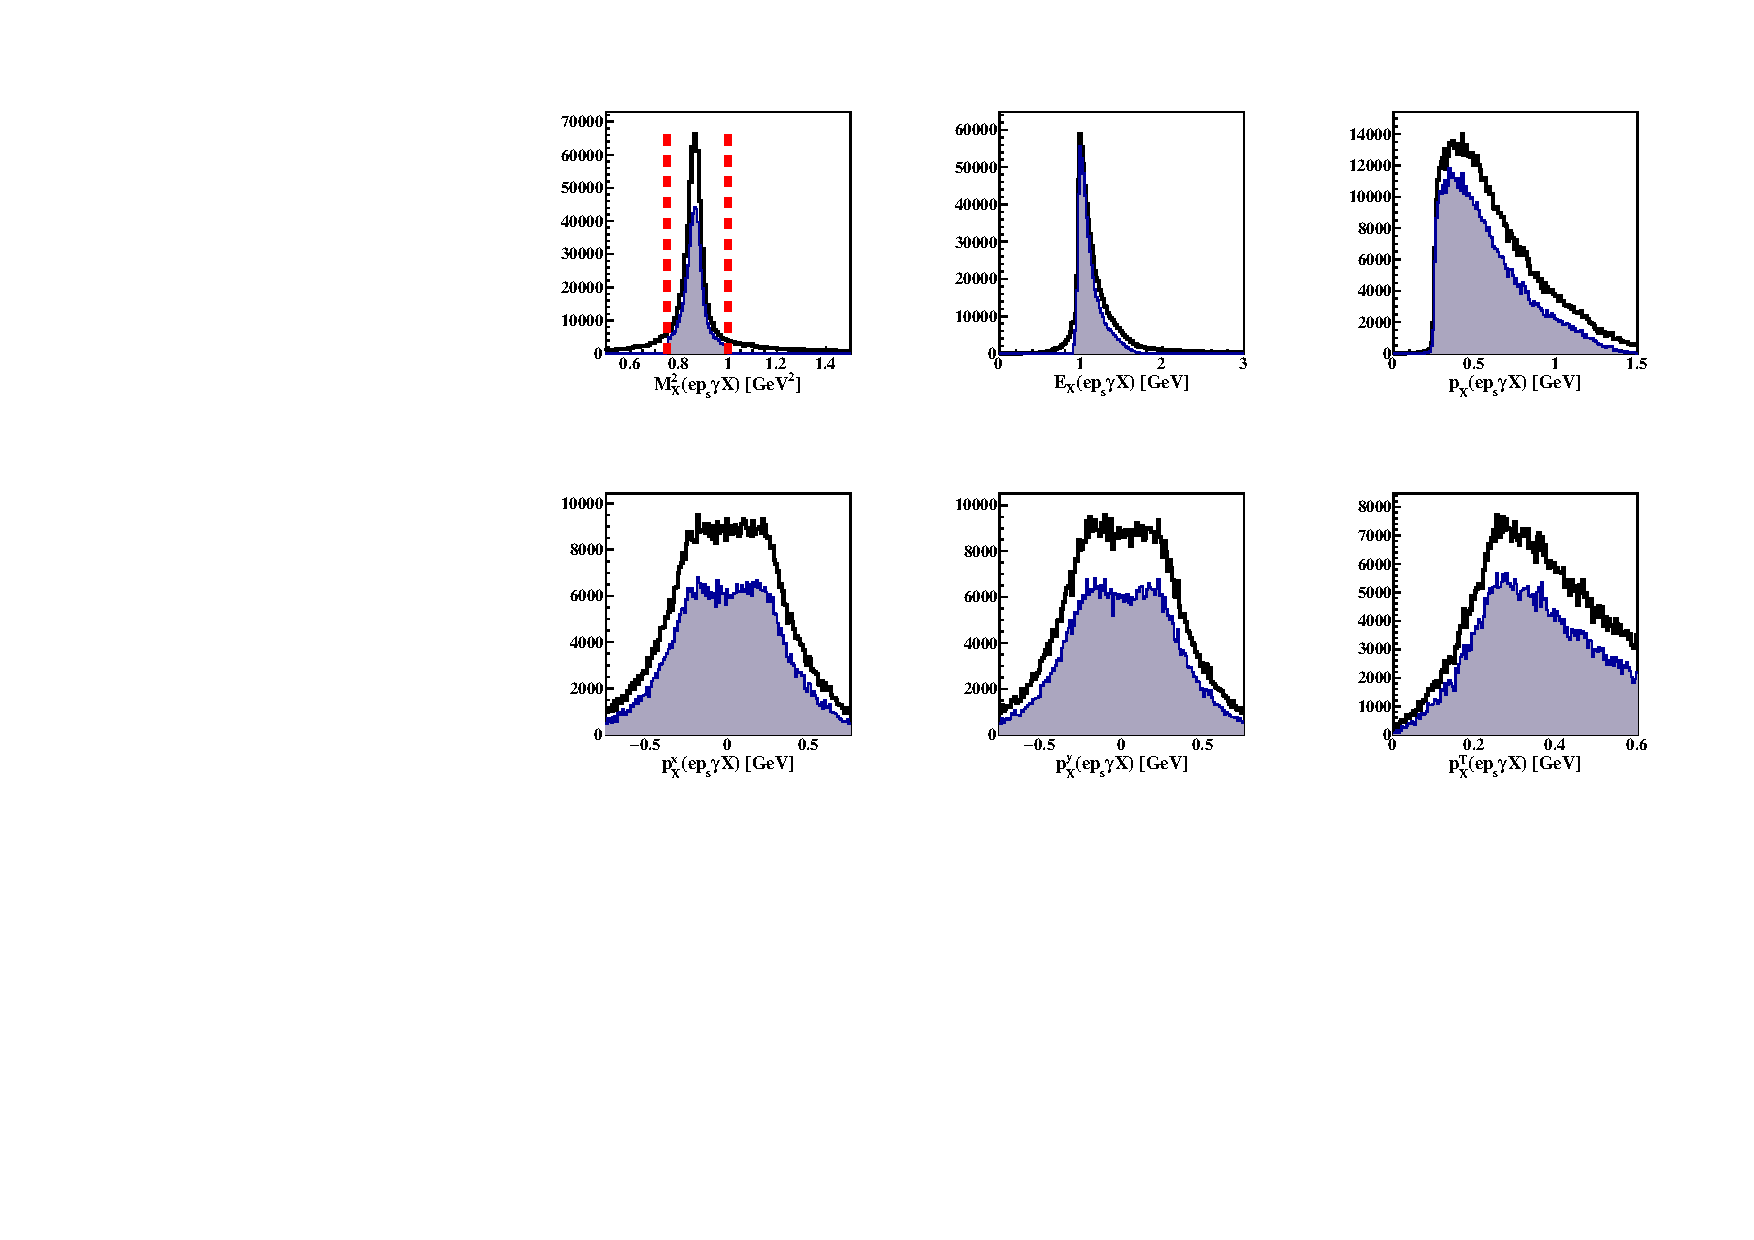
\includegraphics[width=0.95\textwidth,clip]{figs/all_inincoh_exc_cuts.pdf}
  \caption{The distributions of the missing mass squared (left) and the missing 
   energy (right) of the identified Tagged neutron DVCS events. The DVCS 
   exclusivity cuts are represented by the vertical red-dashed lines. The black 
   distributions represent the incoherent DVCS event candidates before the 
   exclusivity cut. The shaded distributions represent the DVCS events that 
   passed the cut on the missing mass squared.
   \label{fig:tagged_exclusive}}
\end{figure}

The spectator approximation assumes that the recoil proton is on its mass shell 
when the electron strikes the neutron and it gains neither energy nor momentum 
in during the interaction. 
In order to study the effect of Fermi motion on our measured DVCS observable, 
we specifically use the kinematics of the photons to determine the transferred 
momentum squared $t$.  Figure~\ref{fig:binning_x_t} shows the distribution of 
$Q^2$ as a function of $x^*$ and $x^*$ as a function of $t$ of the identified 
tagged neutron DVCS events. On the right side plot of 
figure~\ref{fig:binning_x_t} we show the proposed binning in $x^{*}$ versus 
$-t$ space. The data will be binned three-dimensionally into 108 bins. That is, 
12 bins in $x^{*}$ vs. $-t$, and then nine bins in the azimuthal angle ($\phi$) 
for each of the 12 bins. The data are integrated over the full measured range 
of $Q^2$.   
   

\begin{figure}[htb]
  \centering
    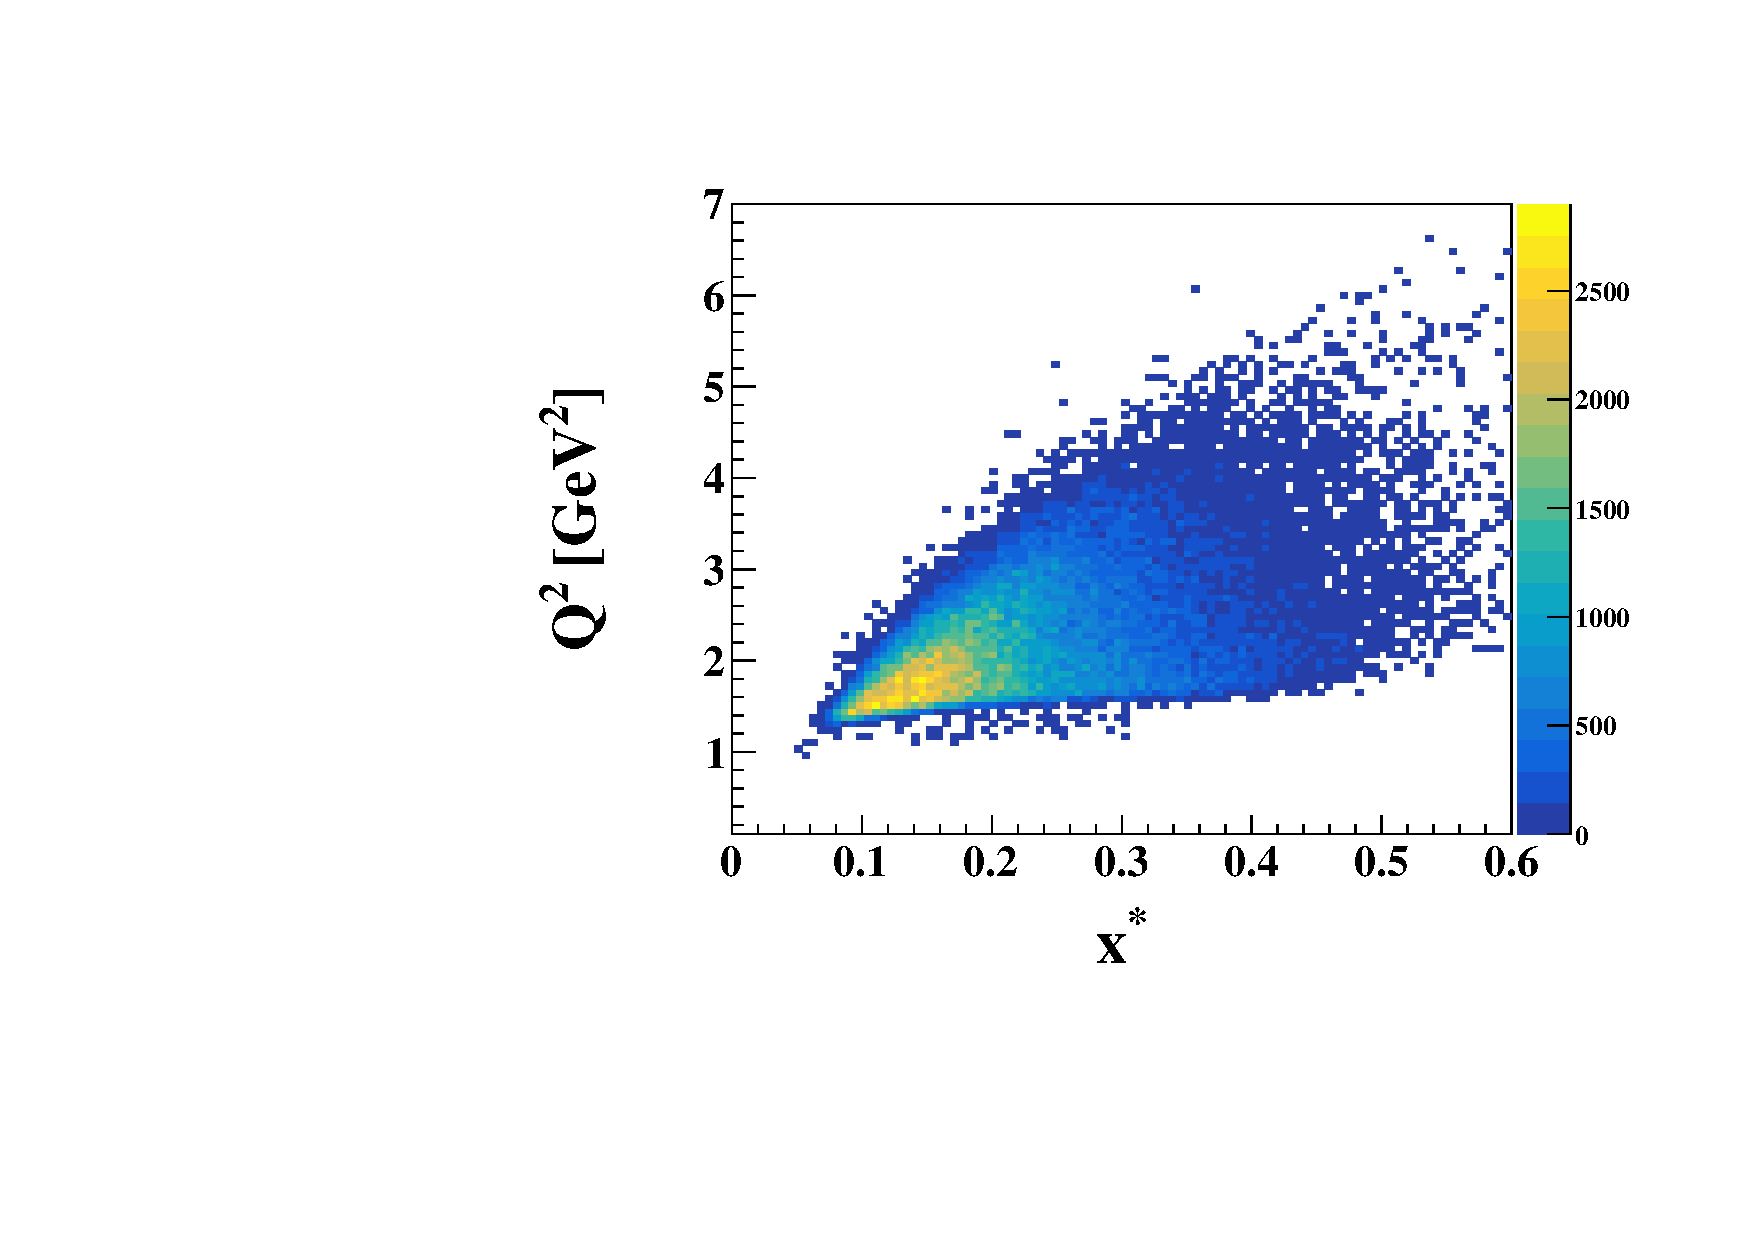
\includegraphics[width=0.45\textwidth,clip]{figs/pdf/Q2_x*.pdf}
    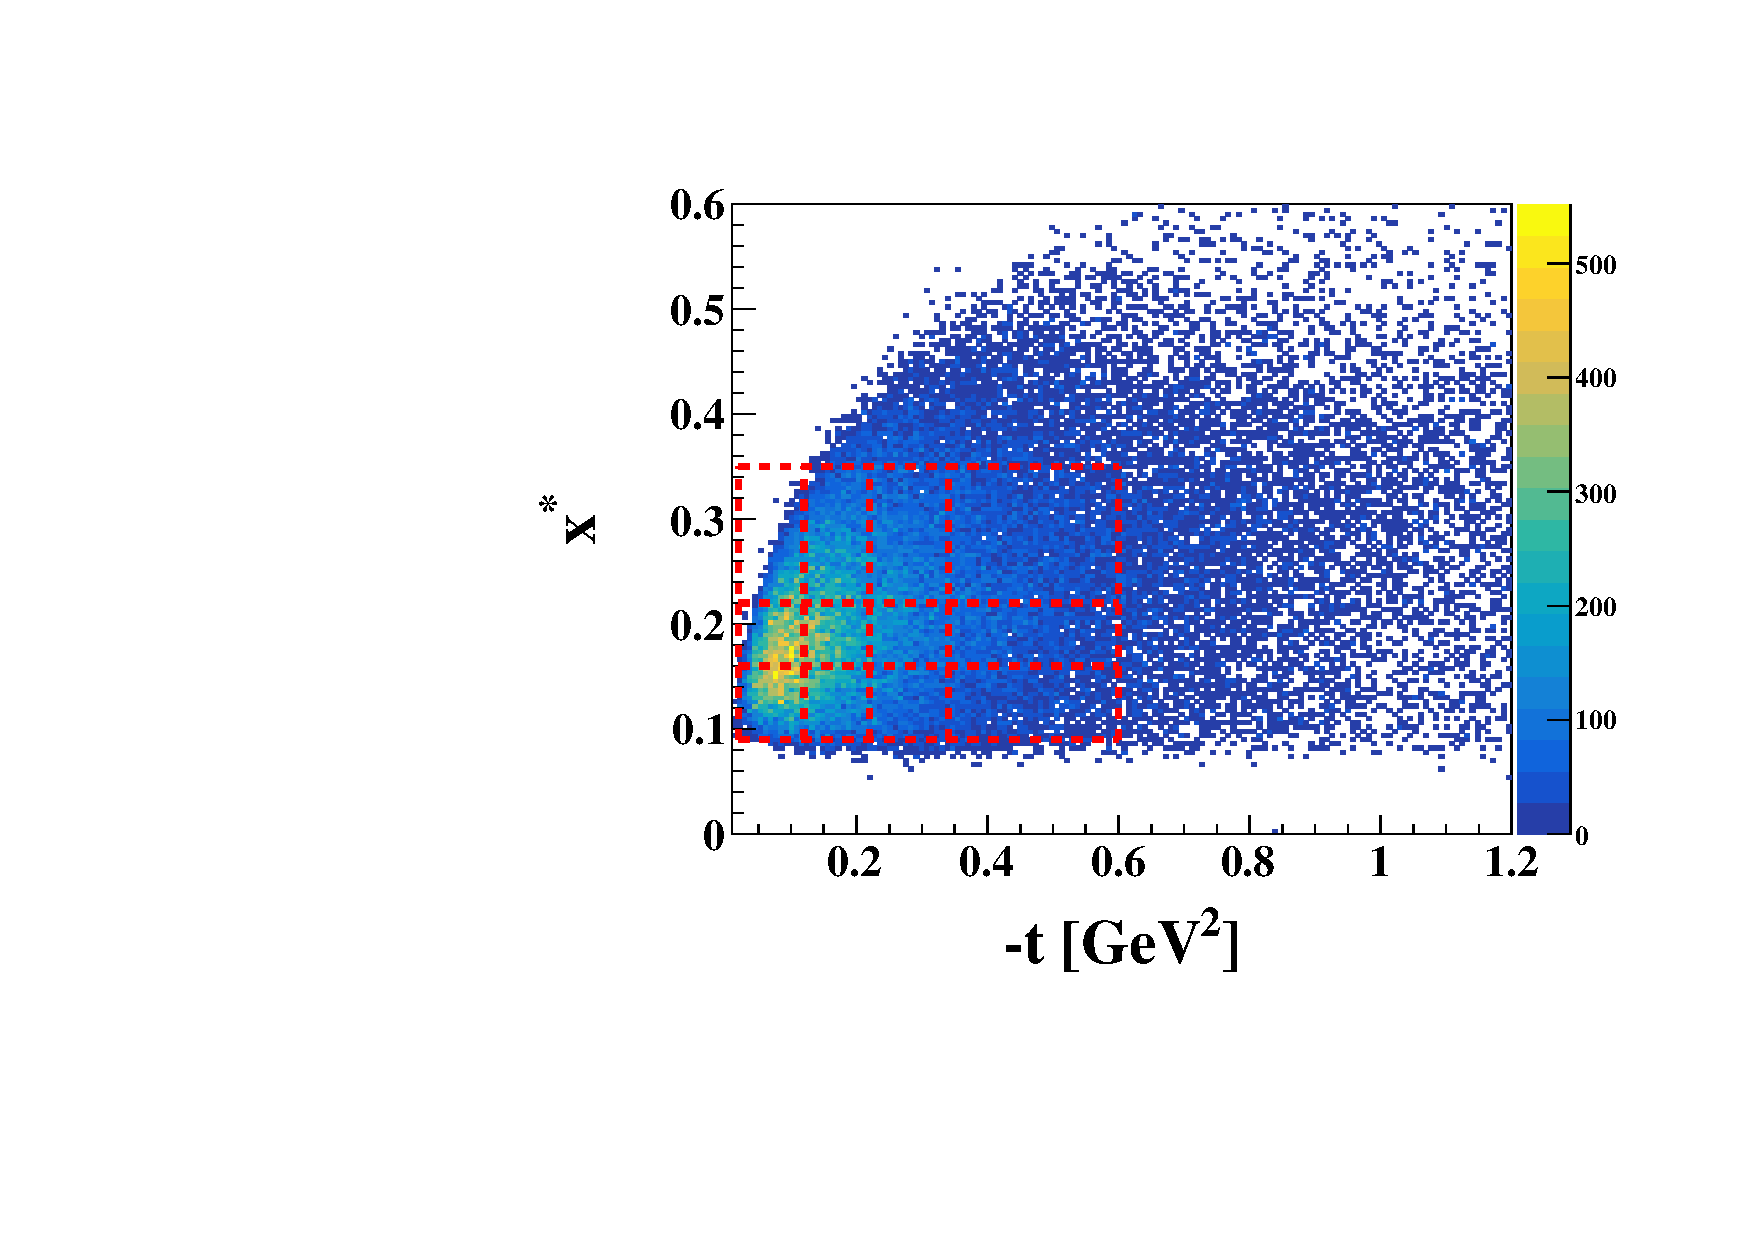
\includegraphics[width=0.45\textwidth,clip]{figs/pdf/t_x*.pdf}
   \caption{The distributions of the tagged neutron DVCS events in terms of 
   $Q^2$ versus $x^*$ (left) and  $x^{*}$ versus $-t$ (right). On the right we 
   show the binning we proposed in $x^{*}$ versus $-t$ space.
   \label{fig:binning_x_t}}
\end{figure}


Figure~\ref{fig:alu_tagged} presents the reconstructed tagged neutron DVCS  
$A_{LU}$ as a function of $\phi$ in bins of $x^{*}$ vs $-t$.  

\begin{figure}[htb]
  \centering
    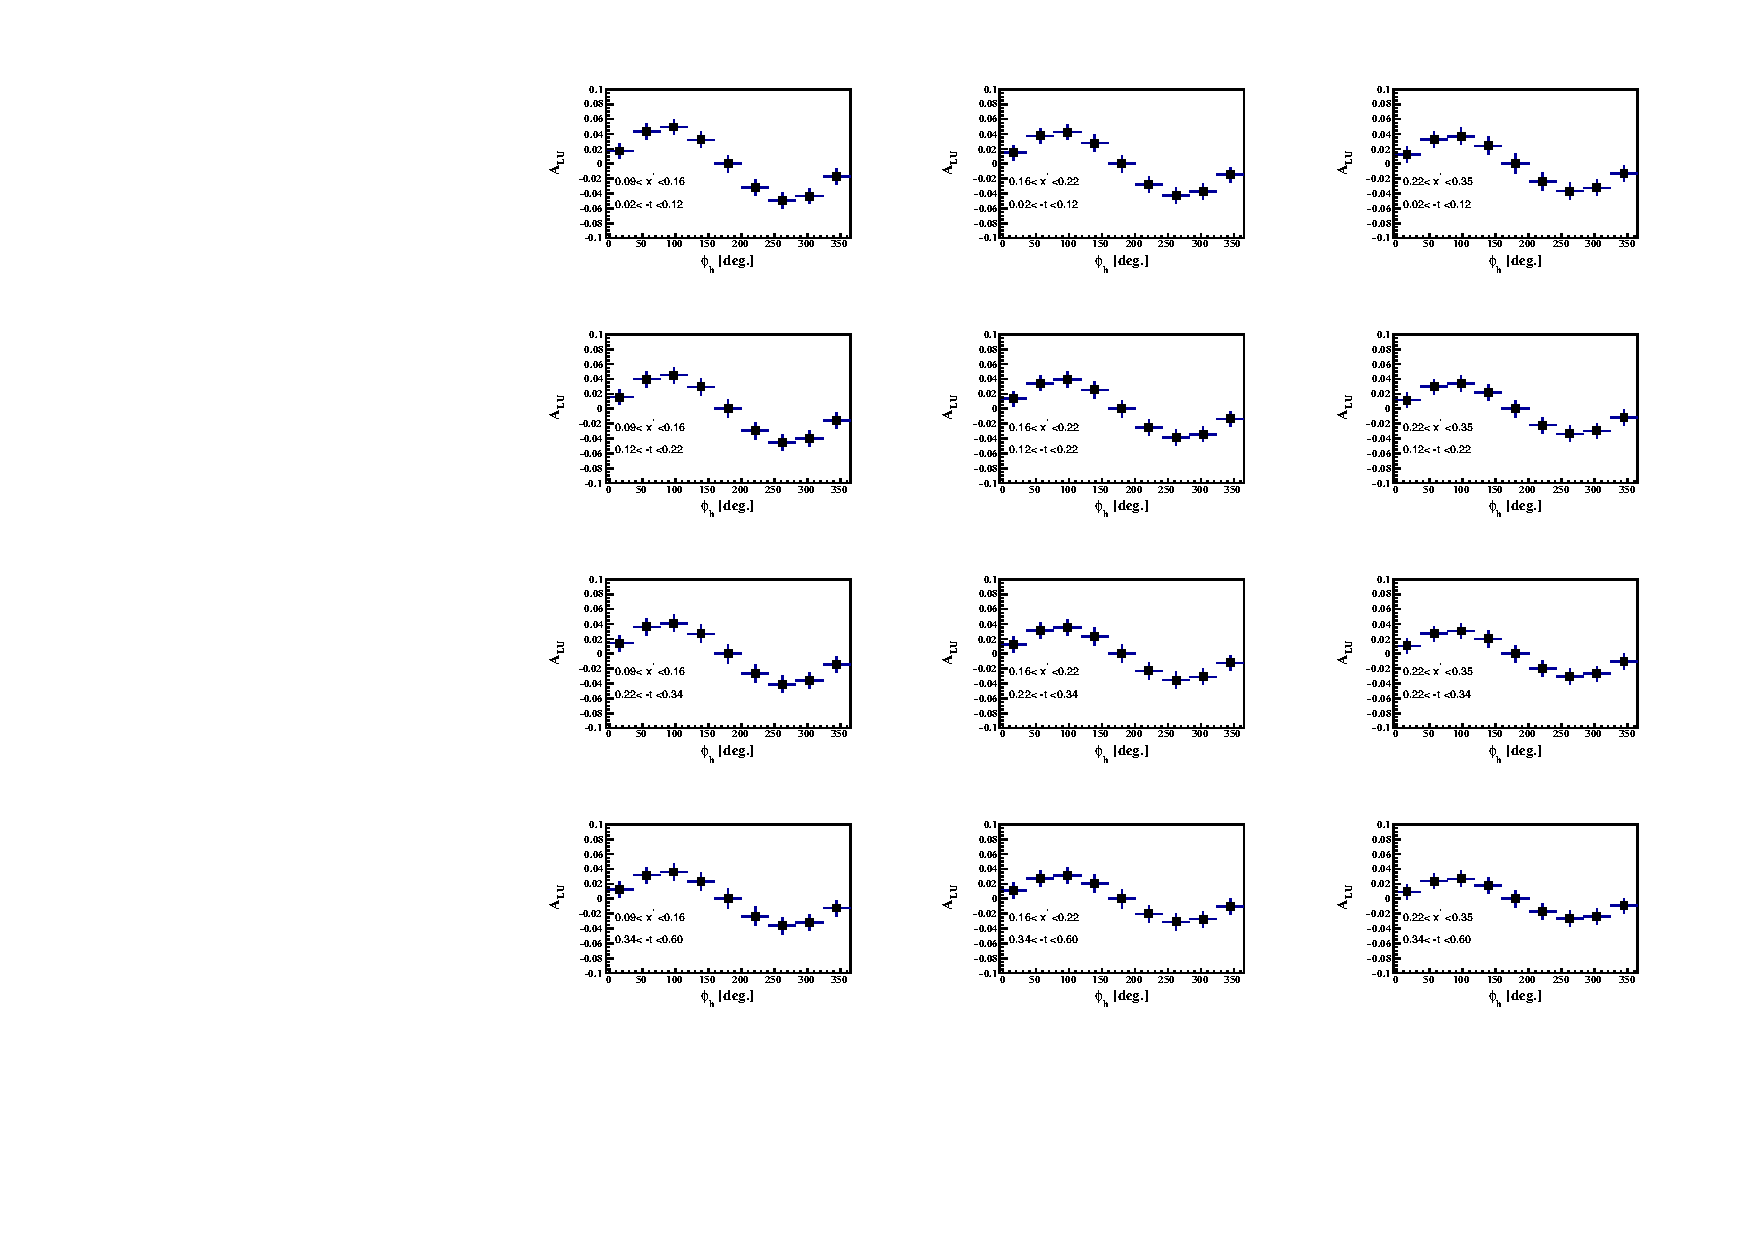
\includegraphics[width=1.1\textwidth,clip]{figs/pdf/BSA_incoherent_Phi_x_t.pdf}
  \caption{Projected beam-spin asymmetries as a function of the hadronic angle 
   $\phi_h$ in the binning of $x^{*}$ vs $-t$ space. The error bars include 
   both the statistical and the systematic uncertainties added quadratically.
   \label{fig:alu_tagged}}
\end{figure}




\subsection{Fully exclusive n-DVCS projections}
Our aim of this measurement is to investigate the Fermi motion and the final 
state interaction (FSI) effects on the measured neutron DVCS beam-spin 
asymmetry. This can be achieved by comparing the measured tagged neutron DVCS 
beam-spin asymmetry, that is by measuring $d(e,e'p_s\gamma)X$, to the measured 
full exclusive neutron DVCS channel, that is by measuring $d(e,e'np_s\gamma)$.  
The selection of the tagged DVCS events have been presented in the previous 
subsection, while different way of binning the data will be constructed as will 
be shown in this section. 

Regarding the fully exclusive neutron DVCS events selection, events with the 
four final state particles being identified after applying all the geometry and 
physics cuts on the individual final state particle. After identifying these 
events, the exclusivity of the DVCS events is ensured by imposing a set of 
constraints based on the four-momentum conservation in the reaction 
$ed\rightarrow e'p_{s}n\gamma$.  The distributions for the exclusive variables 
are shown in figure~\ref{fig:fully_exclusive}.

\begin{figure}[htb]
  \centering
    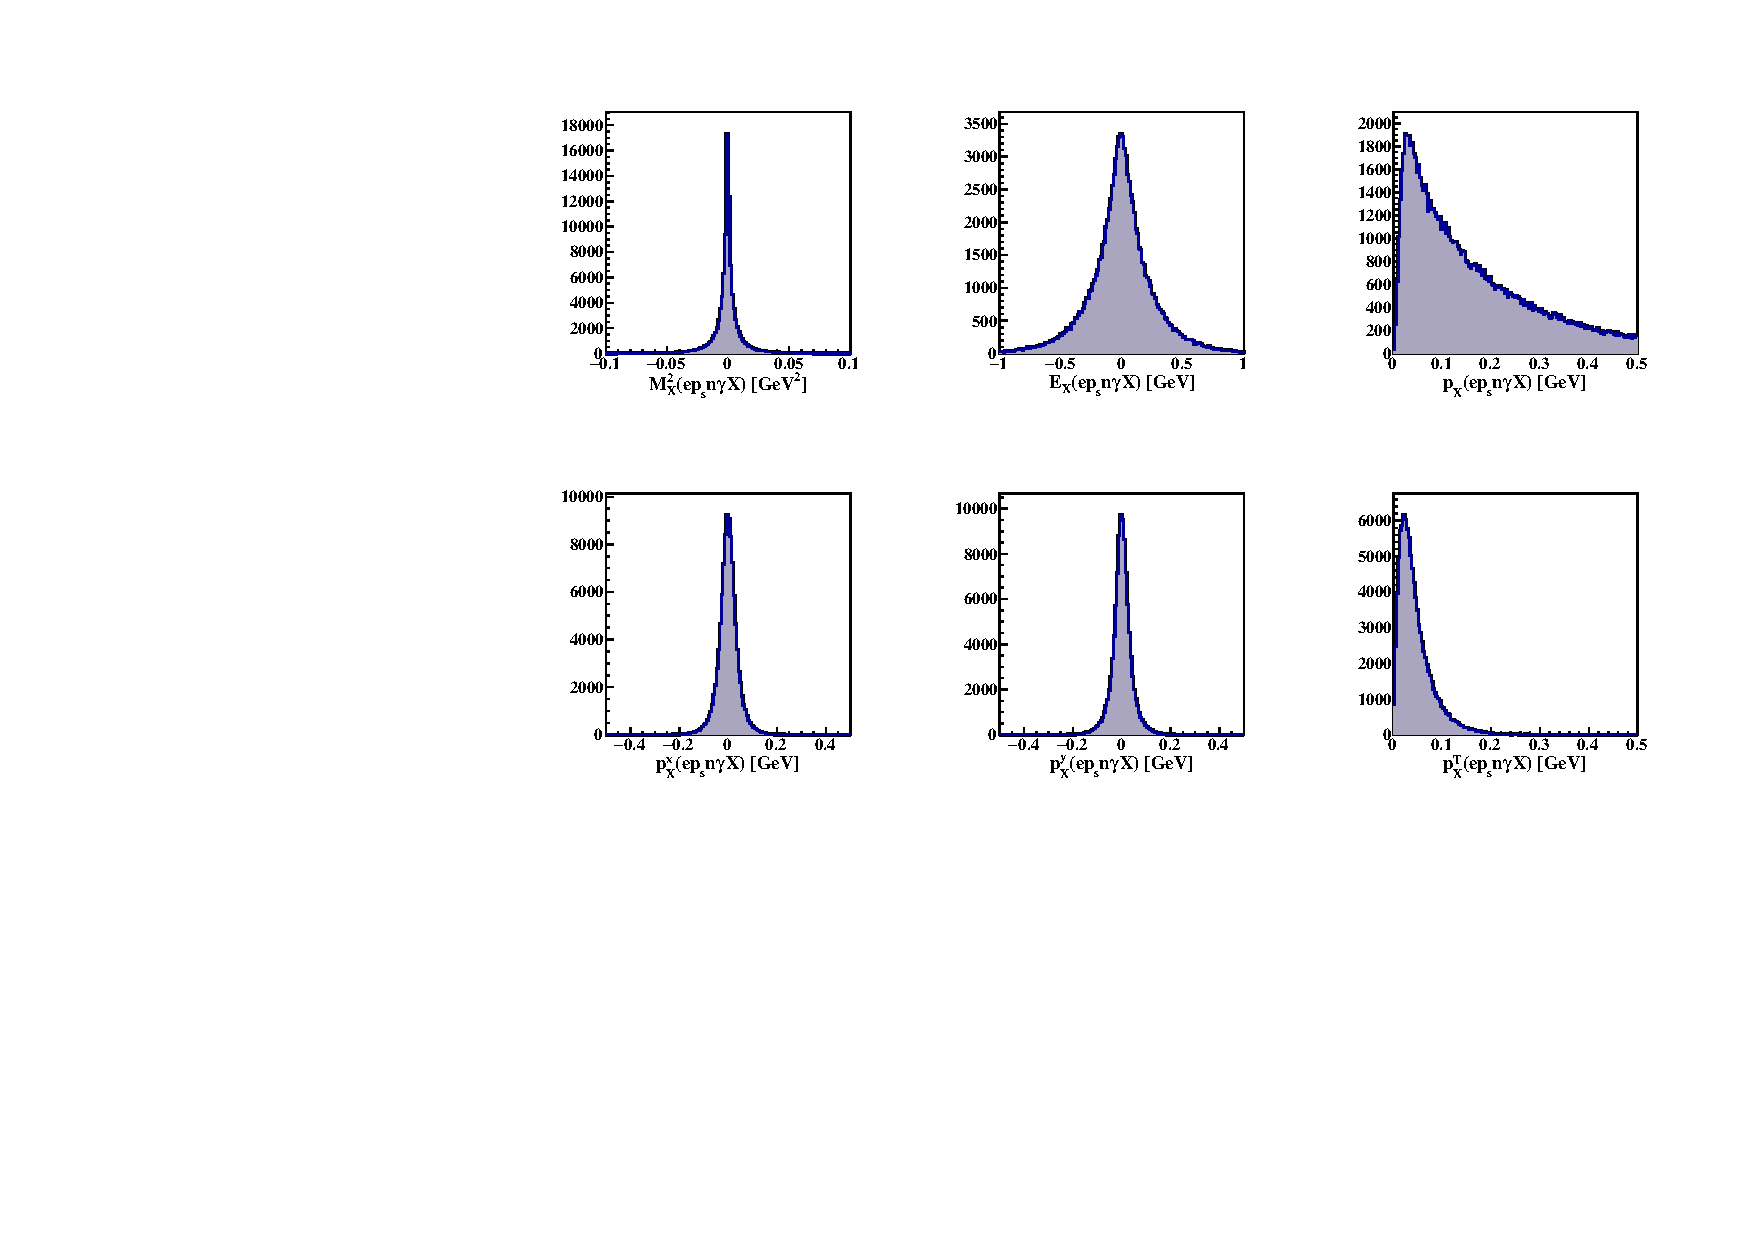
\includegraphics[width=0.95\textwidth,clip]{figs_epngamma/pdf/epngamma_all_incoh_exc_cuts.pdf}
  \caption{
    The distributions from left to right and from top to bottom are:
    missing mass squared, missing energy, missing total momentum, the 
    x-component of the missing momentum, the y-component, and the transverse 
    missing momentum in the $e'p_{s}n\gamma$ final-state system. The DVCS 
    exclusivity cuts are represented by the vertical red-dashed lines. The 
    black distributions represent the DVCS event candidates before the 
    exclusivity cuts. The shaded distributions represent the DVCS events that 
    passed all of these cuts.
   \label{fig:fully_exclusive}}
\end{figure}

As mentioned previously, a total of 850K fully exclusive events will be 
collected within the approved running luminosity and experimental setup of Run 
Group F. Similarly to the tagged DVCS events, we use the kinematics of the 
detected spectator proton to define the modified Lorentz invariant, $x^*$, and 
we define the transferred momentum squared, $t$, using the photons to 
investigate the initial Fermi motion effect on our DVCS observable of interest, 
$A_{LU}$. Figure~\ref{fig:exclusive_binning_x_t} shows the distributions of  
$Q^2$ as a function of  $x^*$ and  $x^{*}$ as a function of $-t$ for the 
identified fully exclusive events. Before binning our data in the space of the 
momentum and the polar angle of the detected spectator momentum, we apply an 
initial cut on $x^{*}$ vs. $-t$, as can be seen in 
Figure~\ref{fig:exclusive_binning_x_t} which stands for the fully exclusive 
detected n-DVCS events. Similar cut is applied on the $x^{*}$ vs. $-t$ space of 
the tagged n-DVCS events. After that, both data sets are binned into 6 bins in 
the momentum of the spectator proton and its polar angle as shown in 
Figure~\ref{fig:ps_binning_x_t}. Finally, the data of each bin in $p_s$ versus
$\theta_s$ is binned into 9 $\phi$ bins for the fully exclusive events and 12 
$\phi$ bins for the tagged n-DVCS events. The reconstructed $A_{LU}$ is 
presented in Figure~\ref{fig:alu_exclusive} as a function of the hadronic angle 
$\phi$ for the tagged n-DVCS events in black points and for the fully exclusive 
n-DVCS events in blue points. The error bars in these projections include both 
statistical and systematic uncertainties. We are considering 20\% systematic 
uncertainties in our projections here as well. As one can see from our 
projections, the systematic uncertainties have the major contribution in the 
precision of our asymmetries and even with the extremely conservative 
assumption of 20\% consideration, we will observe very precise beam-spin 
asymmetries.        

\begin{figure}[htb]
  \centering
    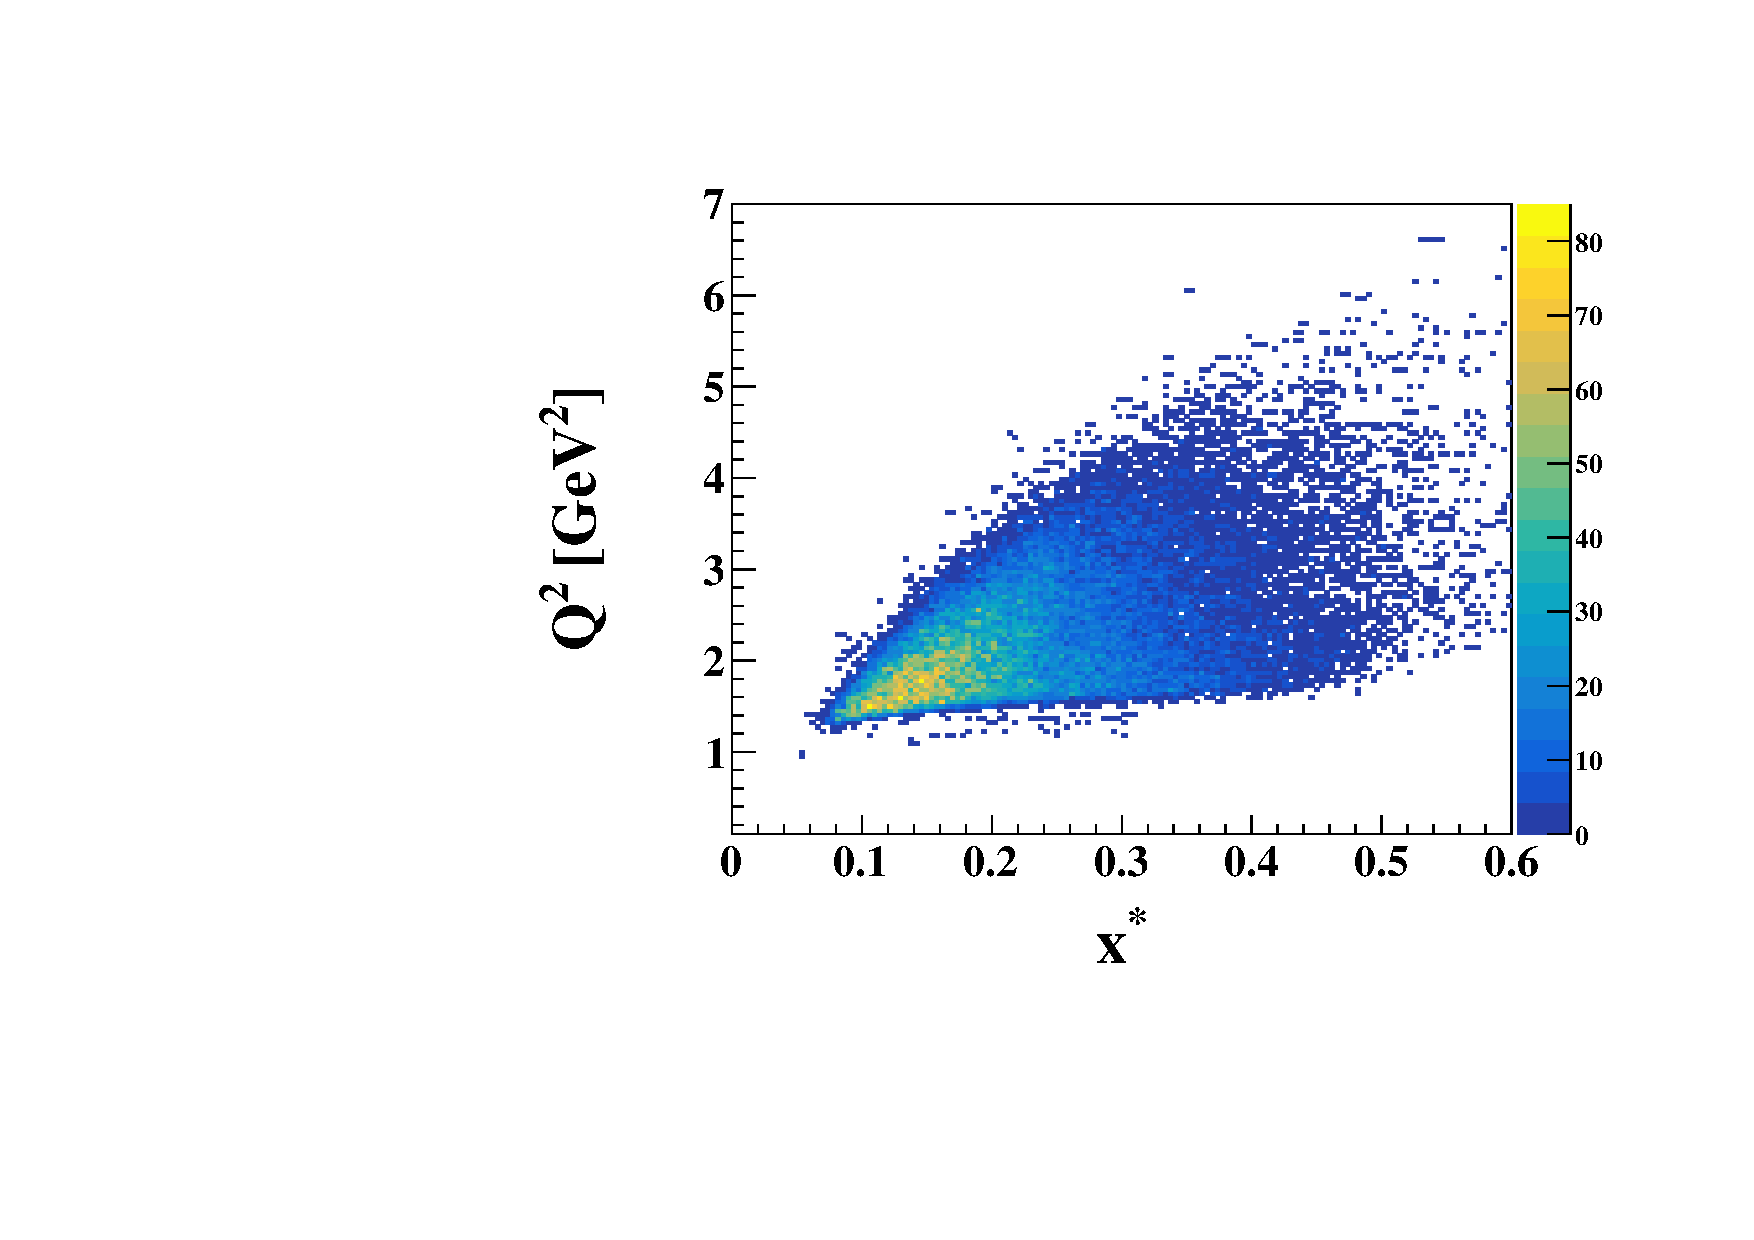
\includegraphics[width=0.45\textwidth,clip]{figs_epngamma/pdf/epngamma_Q2_x*.pdf}
    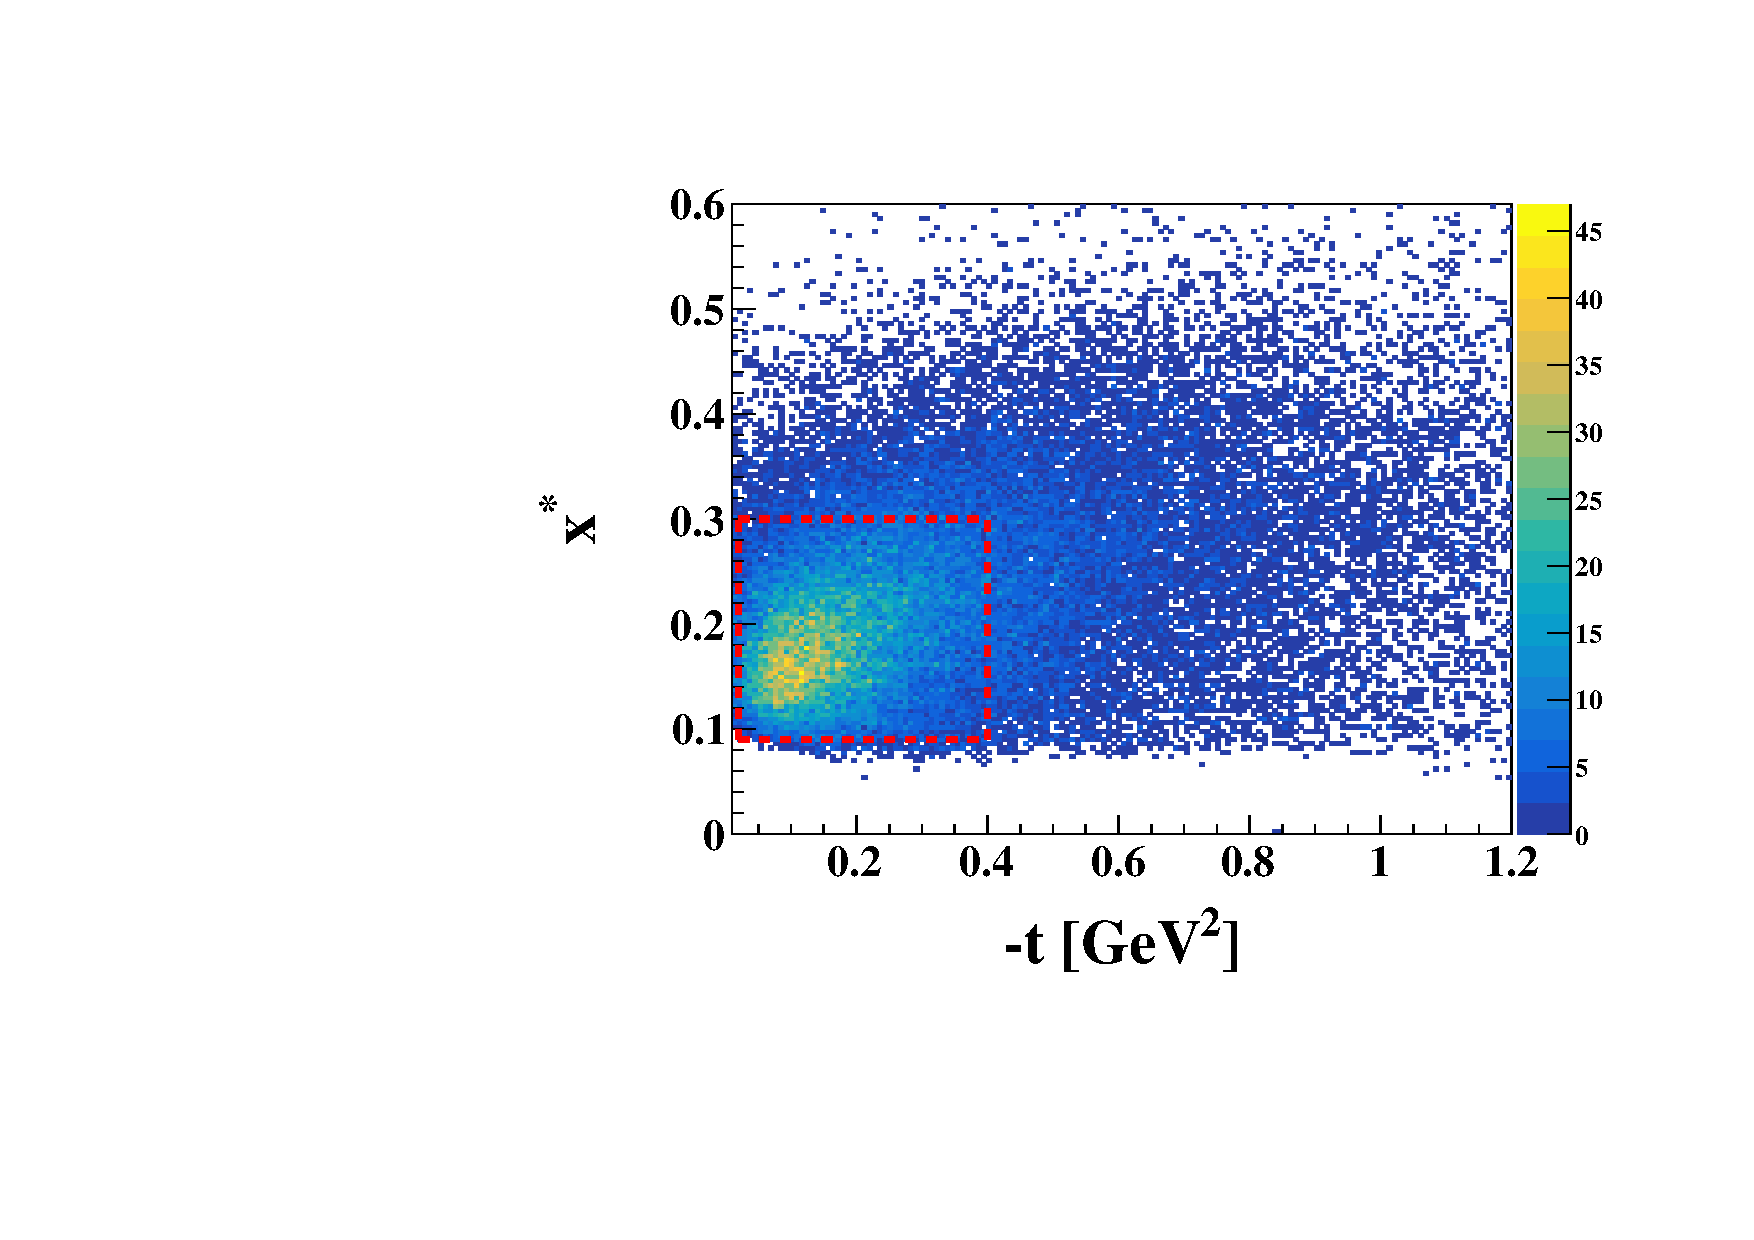
\includegraphics[width=0.45\textwidth,clip]{figs_epngamma/pdf/epngamma_t_x*.pdf}
   \caption{The distributions of the fully exclusive neutron DVCS events in 
   terms of $Q^2$ versus $x^*$ (left) and  $x^{*}$ versus $-t$ (right). On the 
   right we show the bin of interest in $x^{*}$ versus $-t$ space.
   \label{fig:exclusive_binning_x_t}}
\end{figure}



\begin{figure}[htb]
  \centering
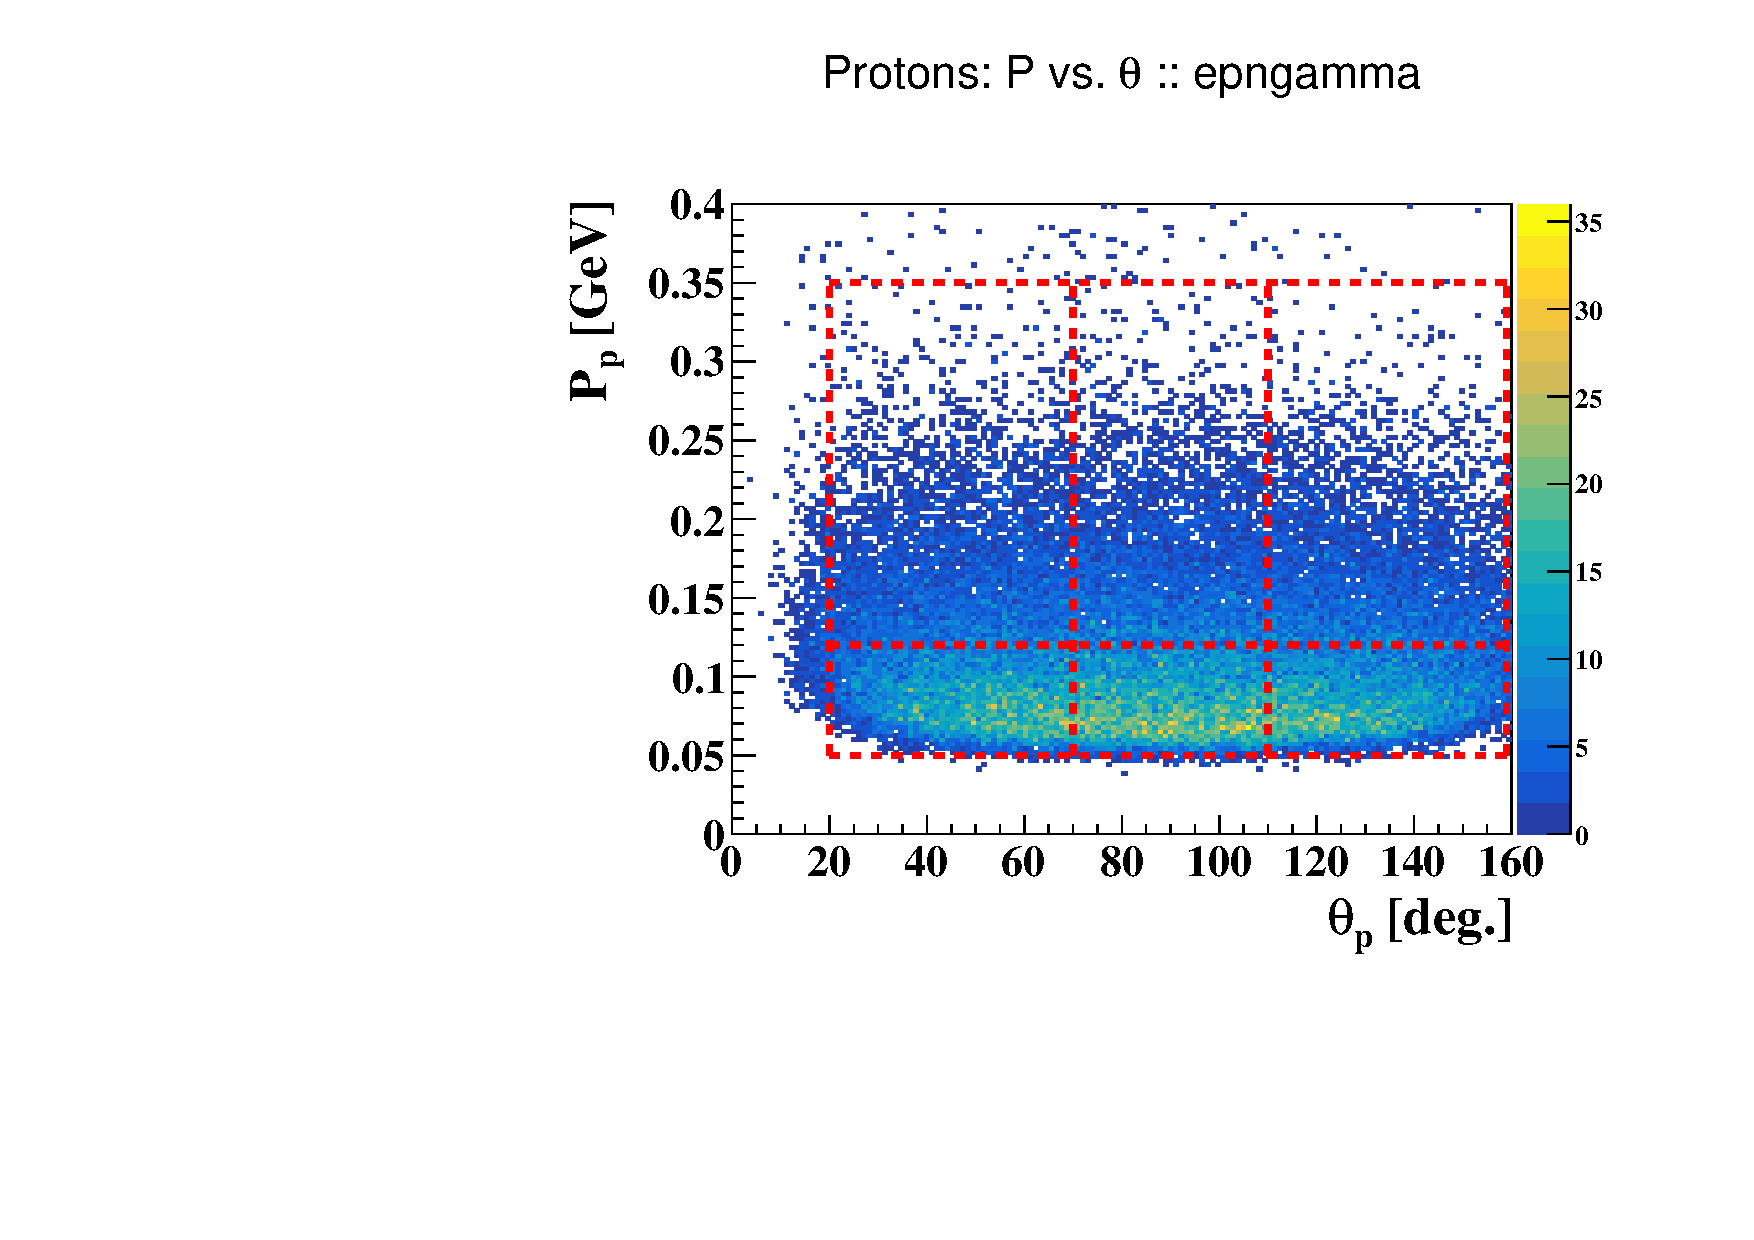
\includegraphics[width=0.55\textwidth,clip,trim=0mm 0mm 0mm 
   20mm]{figs_epngamma/pdf/epngamma_p_p_theta.pdf}
  \caption{Data binning in $p_s$ versus $\theta_s$.
   \label{fig:ps_binning_x_t}}
\end{figure}

\begin{figure}[htb]
  \centering
    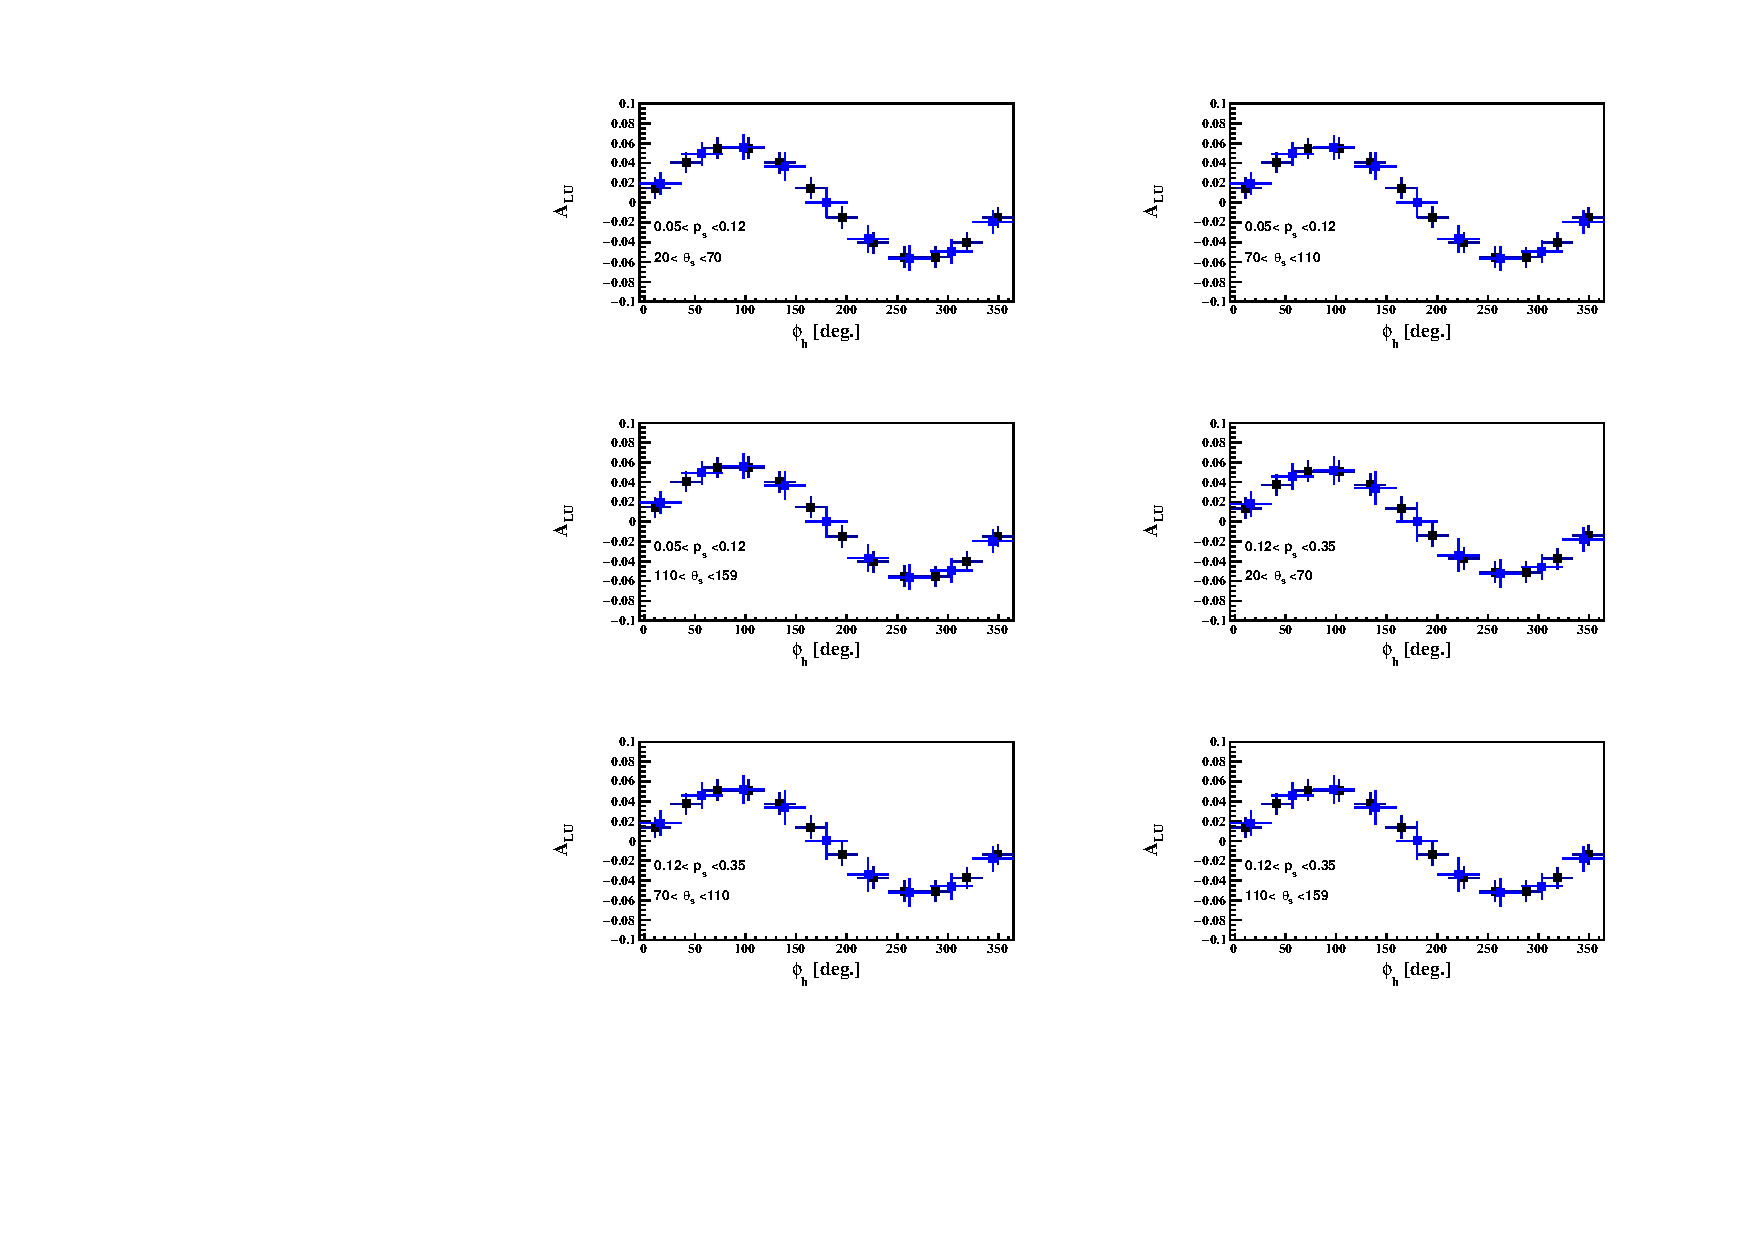
\includegraphics[width=1.1\textwidth,clip]{figs_epngamma/pdf/epngamma_BSA_incoherent_Phi.pdf}
  \caption{Projected beam-spin asymmetries as a function of the hadronic angle 
   $\phi_h$ in the binning of $p_s$ vs $\theta_s$ space. The error bars include 
   both the statistical and the systematic uncertainties added quadratically.
   \label{fig:alu_exclusive}}
\end{figure}



